\begin{figure}[t]
\centering
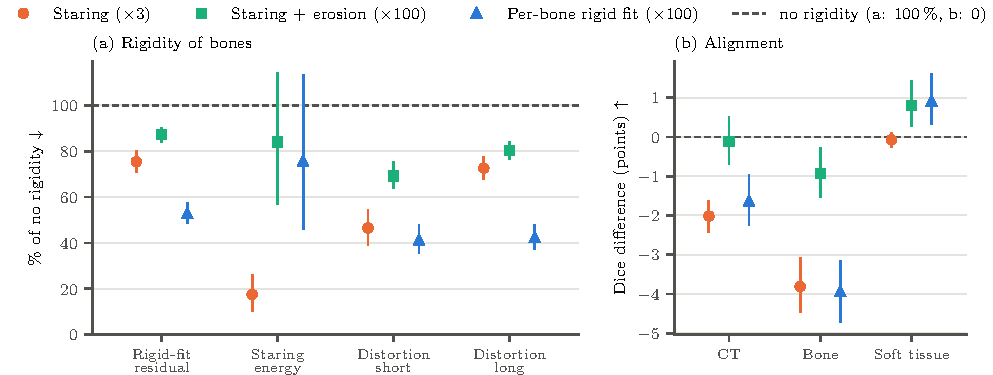
\includegraphics[width=\textwidth]{figures/rigidity_measures.pdf}
\caption{Rigidity penalties evaluated with all rigidity measures on the test set (28 patients, 38 pairs): network trained with the PET losses, followed by instance optimization (IO) with the PET terms and one rigidity penalty at the weight chosen on the validation set.
 (a)~Rigidity of bones relative to IO without rigidity (dashed, 100\,\%), per patient: residual of a rigid fit to each bone (the quantity the rigid-fit penalty minimizes), Staring energy, i.e.\ the Staring penalty (properness, orthonormality, and affinity) on the whole bone (the quantity the Staring penalty minimizes), and the distortion of short (5--15~mm) and long ($\geq$15~mm) within-bone distances (minimized by neither).
 (b)~Change of CT, bone, and soft-tissue Dice relative to IO without rigidity.
 Color and marker shape identify the rigidity penalty.
 Points are means over patients after averaging each patient's pairs; bars are 95\,\% patient-bootstrap confidence intervals.}
\label{fig:rigidity_measures}
\end{figure}
